\chapter{Background}\label{ch:background}
This chapter provides the theoretical foundations for the work presented in this thesis. It introduces the three main concepts which the thesis builds on, power grid operation, reinforcement learning and benchmarking. Section \ref{sec:power_grid_op} explains the fundamentals of electric circuits and how power grids are structured and operated. Section \ref{sec:rl} introduces reinforcement learning and relevant algorithms of it. Finally, Section \ref{sec:benchmarks} focusses on the definition and structure of benchmarks and what good principles are when creating them.



% ============================================================
% ============================================================
\section{Power Grid Operation}\label{sec:power_grid_op}
Power grids are complex systems that, to this date, require human experts from \ac{tso} organisations to operate on them \cite{pptopogym}. They are highly sensitive systems in which the state of numerous components changes within fractions of a second. At the same time, they are indispensable to modern society because most critical infrastructure depends on a reliable electricity supply.

As well as being important to society, power grids are costly to operate and maintain. Operational errors can damage expensive equipment and, in the worst case, cause the entire system to collapse. For example, if their physical limits are exceeded, transmission lines may overheat, which restricts the amount of power that can be generated. This consequently leads to higher operational costs and a greater environmental impact. The increasing integration of renewable energy sources into power grids over the past decades \cite{us_epa_power_2022} has further complicated their operation. These sources are inherently harder to predict and disrupt the grid's balance if not managed properly.

This section provides the necessary background information on electric circuits and power grids. It begins in Section \ref{ssec:electric-circuits} with the fundamentals of electric circuits and the process of electric power generation. Building on this, it goes on to introduce the structure and components of power grids in Section \ref{ssec:power-grids}. Finally, in Section \ref{ssec:ctrl-power-grids} it addresses the challenges involved in operating and maintaining a stable power grid, focusing on the key constraints and characteristics of this process. The remainder of this thesis focuses on the transmission grid, as this is the level most relevant to the control tasks discussed in Section \ref{ssec:ctrl-power-grids}.


% ++++++++++++++++++++++++++++++++++++++++++++++++++++++++++++
\subsection{Fundamentals of Electric Circuits}\label{ssec:electric-circuits}
Electricity is the movement of electric charge in conductive materials. One way to describe this is through an analogy with water. For electricity to flow, there must be a material that conducts electricity and through which electricity can flow. In the water analogy, the conductor is represented by a water pipe, through which water flows. 
In this environment, there are multiple base units to measure electricity from.

In electricity there is \textbf{electric charge}, which is measured in coulombs (\textbf{C}) \cite{rl4network_operation}. Electrons carry a negative charge of $1.602 \times 10^{-19}C$; a deficit of electrons gives a positive charge, while a negative charge occurs for a large number of electrons \cite{fundamentals_circuit_analysis}. If a ring were placed around a water pipe and the amount of water passing through the ring per second were measured, the result would be the flow rate. In electricity, this \textbf{current} is the rate at which electric charges flow in a conductor and it is measured in amperes (\textbf{A} or \textbf{I}). One ampere is the flow of one coulomb of charge per second ($C/s$) \cite{fundamentals_circuit_analysis}.

For water to be able to flow, there must be a pressure difference in the water pipe. With a greater pressure difference, more water will flow (e.g. due to a height difference in the pipe) \cite{rl4network_operation}. For current to flow there must be a difference in electric potential between two points, which is called \textbf{voltage} (\textbf{V}) \cite{rl4network_operation}. Voltage, which is the electric potential difference, creates an electric field inside the conductor, which makes charges move and produce current. The higher the potential difference is, the greater is the flow of electric charge in a conductor \cite{fundamentals_e_circuits}.

Some water pipes are smaller than others, which restricts the amount of water flowing through them. 
In electrical circuits \textbf{resistance} (\textbf{R}) limits the flow of current \cite{rl4network_operation}. Materials that conduct electricity poorly have higher resistance, which causes less current to flow in them. For example in glass, electrons do not move easily, hence there is less current and higher resistance. However in copper, electrons move more easily and produce more current, thus resulting in low resistance. In Equation \eqref{eq:resistance} the mathematical form of resistance shows that resistance depends on the cross-sectional area $A$, the length $l$ and resistivity $\rho$ of the conductor \cite{fundamentals_e_circuits}. In the example of copper and glass, copper has a much lower resistivity of $1.72 \times 10^{-8}$, while glass has a resistivity of $10^{12}$ \cite{fundamentals_e_circuits}. The length of a conductor also affects the resistance, which is a problem that power grids have, as some transmission lines are multiple kilometres long \cite{hvdcReviewIEEE}.

\begin{equation}\label{eq:resistance}
    R = \rho\frac{l}{A}
\end{equation}

\subsubsection{AC and DC Electrical Systems}
In an electrical system, current and voltage behave in two different ways. The simplest way is \ac{dc}, where the electric current flows in one constant direction. In this system the voltage is either constant or has a slow variation over time \cite{fundamentals_e_circuits}. An example of this is a battery, as it provides a fixed voltage, where electrons flow continuously from the negative terminal into the circuit and back to the positive terminal of the battery \cite{distributed_power_generation}. In the other way, in \ac{ac}, voltage and current are time-varying sinusoidal signals. They do not have fixed values like in \ac{dc}, as they change over time in a periodic way. An \ac{ac} system has a frequency, which indicates the number of oscillations per second in the sinusoidal waveform \cite{fundamentals_e_circuits}. In theory \ac{dc} electrical systems also behave as a sinusoidal wave, but the frequency is typically around 0 Hz, which makes the voltage and current stay at a fixed value \cite{fundamentals_e_circuits}.

\subsubsection{Types of Power}
In physics, power defines the rate at which energy is delivered. In electric circuits there are two types of power, active and reactive power. 
\textbf{Active power} is the power that performs useful work, such as mechanical motion, heat, or the generation of light. It is measured in watts (\textbf{W}), which is equivalent to $J/s$ (joules per second) \cite{fundamentals_circuit_analysis}.

In \ac{ac} systems, voltage and current can be shifted in time relative to each other. This shift is described by the phase angle $\phi$ between their sinusoidal waveforms. If voltage and current are perfectly in phase, all transferred power is active power. However, components such as inductors and capacitors cause a phase shift because they temporarily store energy in magnetic or electric fields and later return this energy to the circuit. The resulting cyclic exchange of energy is represented by \textbf{reactive power} $Q$ \cite{fundamentals_e_circuits,power_sys_analysis}. Reactive power is measured in volt-amperes reactive (\textbf{VAR}) \cite{power_sys_analysis}. It does not perform useful work at a load in the same way as active power. Nevertheless, current associated with reactive power still flows through the electrical network. Therefore, reactive power contributes to the total current carried by transmission lines and electrical equipment \cite{power_sys_analysis}.

Active and reactive power can be combined using \textbf{complex power}, as shown in 
Equation \eqref{eq:complex-power}, where $P$ is active power and $Q$ is reactive power.

\begin{equation}\label{eq:complex-power}
\mathbf{S} = P + jQ,
\end{equation}

The magnitude of the complex power is the \textbf{apparent power}, which is measured in volt-amperes (\textbf{VA}). For sinusoidal voltages and current, the three quantities of active power, reactive power and apparent power can be expressed using their 
\ac{rms} values as shown in Equation \eqref{eq:three-powers} \cite{power_sys_analysis,fundamentals_e_circuits}.

\begin{equation}\label{eq:three-powers}
\begin{aligned}
P &= V_{\mathrm{rms}} I_{\mathrm{rms}} \cos(\phi), \\
Q &= V_{\mathrm{rms}} I_{\mathrm{rms}} \sin(\phi), \\
|S| &= V_{\mathrm{rms}} I_{\mathrm{rms}} = \sqrt{P^2 + Q^2}.
\end{aligned}
\end{equation}

When current flows in a resistor, part of the electrical energy is converted to heat, which is called \textbf{dissipated power}. Equation \eqref{eq:heat_power_dc} and Equation \eqref{eq:heat_power_ac} show how dissipated power is defined for \ac{dc} and \ac{ac} electrical systems. They use $V = IR$, which is known as Ohm's law \cite{rl4network_operation}. Both equations are important formulas for power grids, as power lines overheat when the current becomes too high, which damages the grid. Furthermore, the formula shows that increasing the current has a significant impact on the lines as it is proportional to the square of the current. 

\begin{equation}\label{eq:heat_power_dc}
    \begin{aligned}
        P &= VI, \qquad\qquad V = IR \qquad\qquad\Rightarrow\qquad P = I^2R
    \end{aligned}
\end{equation}

\begin{equation}\label{eq:heat_power_ac}
    \begin{aligned}
        P &= \frac{1}{2}V_{max}I_{max}, \qquad V = IR \qquad\Rightarrow\qquad P = \frac{1}{2}I_{max}^2R
    \end{aligned}
\end{equation}

Over long distances, electrical power is transported at higher voltage to reduce the current flowing in the transmission lines \cite{rl4network_operation}. Equation \eqref{eq:high_voltage_low_current} shows for \ac{dc} electrical systems why this is the case. Increasing the voltage proportionally reduces the current. Thus, the higher the voltage, the lower the current, and the heat loss drops quadratically, leaving the power line in a stable state without overheating. Maintaining a high level of voltage for each conductor is essential to ensure a sustainable flow of current \cite{rl4network_operation}. The same applies to \ac{ac} electrical systems, where maintaining voltage levels within acceptable limits is crucial for a stable power grid. 

Another challenge with \ac{ac} systems is that a large amount of reactive power increases the line's current, even when the active power stays the same. For this reason control over the reactive power is also important for a stable grid \cite{power_sys_analysis}.

\begin{equation}\label{eq:high_voltage_low_current}
    \begin{aligned}
    P_{total} = VI \qquad\Rightarrow\qquad I = \frac{P_{total}}{V}\\
    P_{loss} = I^2R = (\frac{P_{total}}{V})^{2}R
    \end{aligned}
\end{equation}

\subsubsection{Electric Power Generation}
There are multiple steps that lead to electric power generation. It begins with a primary energy source, such as fossil fuels (e.g. coal and gas), nuclear energy, water flow, wind and solar radiation \cite{power_sys_analysis}. This primary energy is converted into electric energy. To achieve this, most power plants convert the energy first into mechanical energy, e.g. through steam turbines in thermal plants, water turbines in hydropower plants and wind turbines in wind parks \cite{electircal_machines}. Based on electromagnetic induction, the generator converts mechanical energy into electrical energy in the form of alternating current and voltage \cite{electircal_machines}.


% ++++++++++++++++++++++++++++++++++++++++++++++++++++++++++++
\subsection{Power Grids}\label{ssec:power-grids}
A power grid is a network that transports electricity from multiple sources to multiple loads. It consists of \textbf{generators}, which provide the power, \textbf{transmission lines}, that connect the whole grid, and \textbf{loads}, or power sinks, which consume the generated electricity. Between the generators and loads, \textbf{substations} are the intermediate grid nodes. Through the connected transmission lines, the power flows from generators, to substations and then it reaches the loads. Another important component is \textbf{transformers}, which regulate the voltage levels \cite{rl4network_operation}.

Figure \ref{fig:simple_power_network} shows a simple power grid, with two generators (denoted g), three loads (denoted c), five substations (denoted s) and network lines (denoted l) to connect the whole grid. In this grid there are many ways for the electricity to flow from generators to loads. For example if the current flowing from generator $g_1$ to load $c_2$ through the lines $l_5$ and $l_6$ is too high, it can also be redirected to other lines, such as line $l_7$, to distribute the current more evenly.

\begin{figure}[htp]
    \centering
    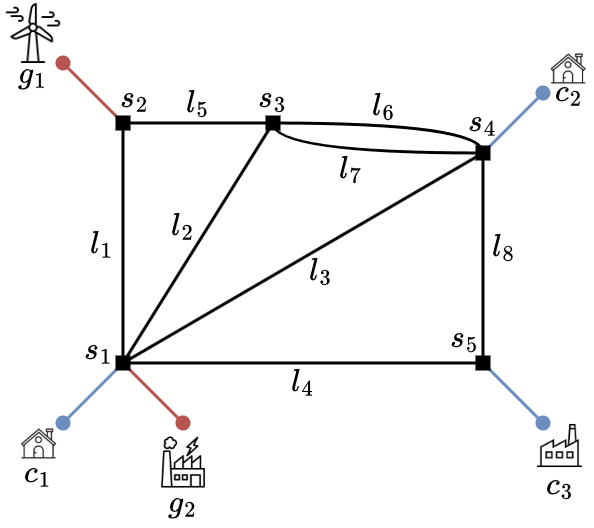
\includegraphics[width=0.45\textwidth]{images/background/simple_power_grid.png}
    \caption{Example of a simple power grid \cite{rl4network_operation}}
    \label{fig:simple_power_network}
\end{figure}

In electrical circuits a set of fundamental rules, called Kirchhoff's laws, define how the electricity flows through them:
\begin{quotation}
    \noindent
    \textbf{Voltage law:} Voltage around any closed loop sums to zero.\\
    \textbf{Current law:} Current entering and exiting any node sums to zero.
\end{quotation}
These laws also apply to power grids, which are essentially large, complex circuits \cite{rl4network_operation}. With the usage of the equations from Section \ref{ssec:electric-circuits} on delivered power, voltages and power loss, and Kirchhoff's laws, the behaviour of the power grid is analysed and predicted.

\subsubsection{Power Grid Components}
Each power grid has a variety of potential power sources. Traditionally, these sources were fuel-based (e.g. coal, natural gas and nuclear), located close to the cities that used them \cite{rl4network_operation}.
In modern power grids, power generation is also done using renewable energy sources, such as solar and wind power \cite{rl4network_operation}. These are often located in places far from any big cities, hence the distances to loads are greater \cite{RoleOfGridExtensionsEurope}. 
The distances between generators and loads are not the only difference with traditional power sources. Renewable energy sources also present a new challenge. 
These power sources are less predictable than traditional ones, as their generation of power relies on weather conditions and other factors \cite{challenges_integrating_var_renewables}. 
Consequently, they will not always produce electricity when it is needed. For example, if the highest power demand in winter occurs in the evening, solar panels are highly unreliable in countries such as those in the Nordic region, where the sun sets early in winter.
The different distances between generators and sources, and the variable power generation and demand, must be managed to maintain a stable power grid.

As already mentioned in Section \ref{ssec:electric-circuits}, for electrical systems there are two types of currents, \ac{ac} and \ac{dc}. When transporting electricity in the power grid with transmission lines, one of those two options has to be used. While \ac{dc} offers constant voltage transmission, \ac{ac} enables voltages to be raised or lowered using power transformers \cite{rl4network_operation}. Both allow high voltage transmission, though the variability of voltages in \ac{ac}, makes the transmission easier to control and less expensive than converters needed in \ac{dc} \cite{hvdcReviewIEEE}. For this reason power grids use mostly \ac{ac} \cite{rl4network_operation}. However, there are some use cases where \ac{dc} is used, such as \ac{hvdc}. In transmissions over far distances, like in submarine cables between countries or when transmitting power from offshore wind farms, \ac{hvdc} offers an advantage \cite{hvdcReviewEnergyWeek}. There is a transmission distance, where the total cost for \ac{dc} is lower than with \ac{ac}. This distance is called the break-even distance and is around 500 to 800km \cite{hvdcReviewIEEE}.
Furthermore, \ac{dc} transmission is used to connect two asynchronous \ac{ac} networks (networks with different frequencies). To make this possible a rectifier converts \ac{ac} to \ac{dc} and an inverter converts \ac{dc} back to \ac{ac} \cite{hvdcReviewEnergyWeek}.

The nodes connecting everything in the power grid are buses. Buses are single, fundamental electrical nodes, representing a single voltage level at a specific location, to which other grid components, like lines, loads or generators are connected \cite{pandapower}. Substations, on the other hand, contain multiple buses that together form a station-level-structure, which can be split or coupled. Splitting a substation means distributing grid components that are connected to the substation across multiple buses \cite{pptopogym}.

The power grid is split into four categories when it comes to the transport of power \cite{us_elec_industry_primer}. 
The \textbf{high voltage transmission grid} and \textbf{transmission grid} operate at high voltages for long-distance transport from large generation sites to regional substations. The high voltage transmission grid works above 765 kV \cite{us_elec_industry_primer}, while the transmission grid is maintained between 100 kV and 765 kV \cite{grl4powergrids}.
The \textbf{sub-transmission grid} is an intermediate layer which connects transmission substations to distribution substations and maintains voltages under 70 kV \cite{us_elec_industry_primer}.
The last layer is the \textbf{distribution grid}, which operates at the lowest voltages to safely deliver power to consumers. It manages voltages under 34 kV \cite{us_elec_industry_primer}. Most households receive power at much lower voltages. For example, households in Europe receive 230 volts and households in North America 120 volts \cite{rl4network_operation}. To ensure safe power delivery to homes, a step-down transformer is required to lower the voltage for local distribution \cite{rl4network_operation}.

Among these four categories, this thesis focuses specifically on the \textbf{transmission grid}, as this is the level at which \acp{tso} (see Section \ref{ssec:ctrl-power-grids}) actively manage power flow and grid stability.


% ++++++++++++++++++++++++++++++++++++++++++++++++++++++++++++
\subsection{Controlling Power Grids}\label{ssec:ctrl-power-grids}
As discussed in the previous sections, power grids contain multiple components. These have constraints, characteristics and behaviours to consider when operating on a power grid. This section presents the key aspects of power grid operation and explains how control centres, operated by \acp{tso}, manage the \textbf{transmission grid} to ensure stability and reliability.

\subsubsection{Constraints and Characteristics of Power Grids}\label{sssec:const_character_pg}
There are three primary constraints to ensure a stable power grid. Firstly, as previously mentioned, heat loss damages the network lines. For this reason the thermal limits of each line must be respected, and the voltage must be kept high to avoid exceeding them. Secondly, the voltage has to be in a correct range, as voltages must be kept high for transmission and lower for delivery to loads. 
Grid voltage must typically remain within $\pm10\%$ of its nominal rated value for low-voltage networks \cite{en50160}, though tighter limits may apply in transmission grids depending on national grid codes \cite{ansi_c84}. This ensures that the equipment operates safely and the power grid remains stable and reliable.
Lastly, generation and load must be balanced at all times. If power generation exceeds demand, then the power grid becomes unstable. Conversely, if there is not enough power to deliver to the loads, then power outages happen. 
Despite these constraints, operating the power grid is a time-domain challenge \cite{rl4network_operation}. Power grids have a brief window in which they can exceed their limits without the system collapsing. Solutions do not have to be implemented immediately when lines are overloaded. A short overload does not result in immediate disconnection, but the aim must always be to keep the grid in a stable state.

In addition to these constraints, the characteristics of power grids must be considered. Firstly, a power grid is a meshed network, meaning it contains many potential network states \cite{grl4powergrids}. The grid contains a number of switchable components, such as lines that are switched in or out of service, and busbars at substations that are split or coupled \cite{rl4network_operation}. These components enable electricity to be redirected and the flow to be controlled. Figure \ref{fig:power_op} illustrates this behaviour, showing the substation $s_3$ being split on two buses, to separate the flow coming from $s_1$ and $s_2$, while the line $l_3$ is out of service. 
Lastly, power grids are static in the sense that network operators cannot create new interconnected elements whenever they are needed. Expanding a power grid is a time-consuming process involving the construction of new grid elements \cite{rl4network_operation}.

\begin{figure}[htp]
    \centering
    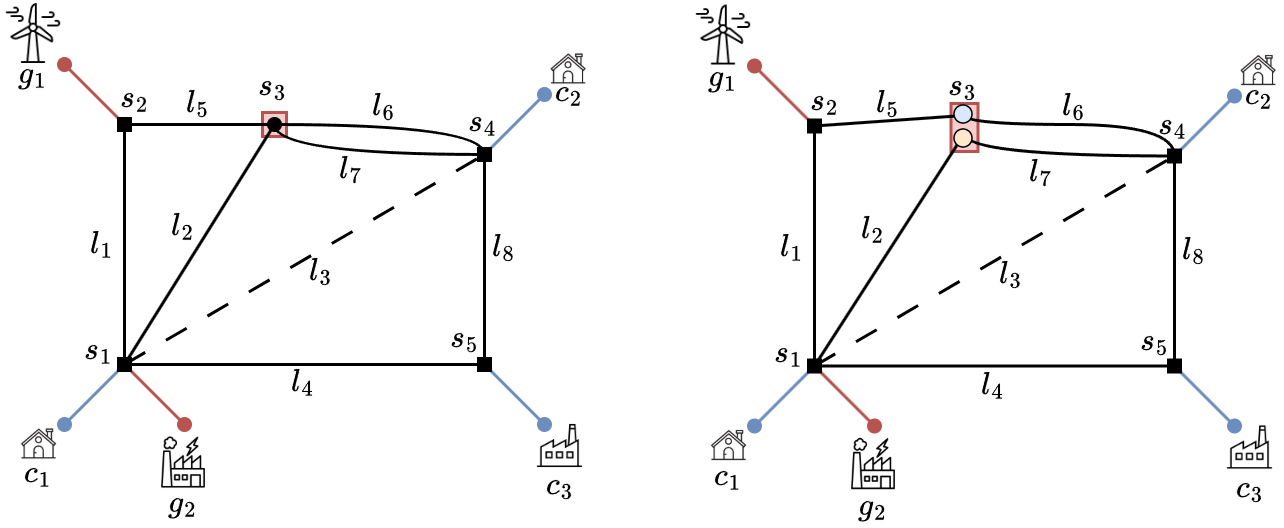
\includegraphics[width=0.9\textwidth]{images/background/power_grid_operation.png}
    \caption{Example of substation splitting and out of service lines (indicated by dotted lines) \cite{rl4network_operation}}
    \label{fig:power_op}
\end{figure}

\subsubsection{Operating on Power Grids}
The \ac{tso} chooses from a handful of actions, to operate on the power grid. The cheapest option is to switch lines in or out of service; splitting or coupling substations is more expensive. Increasing or reducing the output of a generator to adjust the flows on the lines is even worse in terms of costs, as it affects the energy market and increases costs for customers. Disconnecting loads is the most expensive action and should be avoided, as it causes disruptive effects on society, businesses, and people's daily lives \cite{rl4network_operation}. 

The transmission of power grids is controlled from control centres. These centres observe all elements of a grid and control some of them. 
For instance, they have full control over lines and substations via remote commands. Furthermore, they adjust the output of generators through remote instructions. Even some of the loads in a grid are controllable, though most of them are controlled by distribution system operators \cite{rl4network_operation}.

While a small to medium-sized country only has one control centre, larger countries (e.g. USA and Canada) have multiple control centres, which coordinate operations with neighbouring centres \cite{rl4network_operation}. 
These centres work continuously, as they must always comply with the constraints mentioned at the beginning of this section (thermal limits, voltage ranges, and the balance between generators and loads).
To increase the safety in a power grid, these centres must also be able to anticipate contingency states (i.e. states with unexpected failures or losses of key components). Examples of such techniques include $N-1$ or $N-k$ contingency analysis, in which the grid is simulated running with one or k elements removed \cite{nk_outages}. $N-0$ analysis is also used, which would be the base-case power flow simulation analysis, with no elements removed. These analyses enable operators to ensure safer operation even after failures occur.
Another possible situation is that there is a scheduled outage due to grid element maintenance.
Grid operators need to be aware of these situations and also plan for and manage system peaks during the day or during different seasons \cite{rl4network_operation}.



% ============================================================
% ============================================================
\section{Reinforcement Learning}\label{sec:rl}
\ac{rl} is a branch of \ac{ml} in which an agent interacts with an environment and learns to make decisions. Instead of learning from a fixed dataset, in \ac{rl} the agent receives feedback in the form of rewards, which it seeks to optimise. This design makes \ac{rl} particularly suited for solving decision-making problems, such as operating a power grid. This section provides the necessary background on \ac{rl}, by first explaining the fields of \ac{ml} in Section \ref{ssec:fields-learning} and then showing the theory and concrete algorithms of \ac{rl} in Section \ref{ssec:rl-terminology} and Section \ref{ssec:example-agents}. 

% ++++++++++++++++++++++++++++++++++++++++++++++++++++++++++++
\subsection{Fields of Learning}\label{ssec:fields-learning}
In the field of \ac{ml} there are multiple different types of learning. Each of them has different approaches to learning and how they are used varies significantly. While this thesis focusses on \ac{rl}, the fields of supervised and unsupervised learning are related to it.

\begin{figure}[htp]
    \centering
    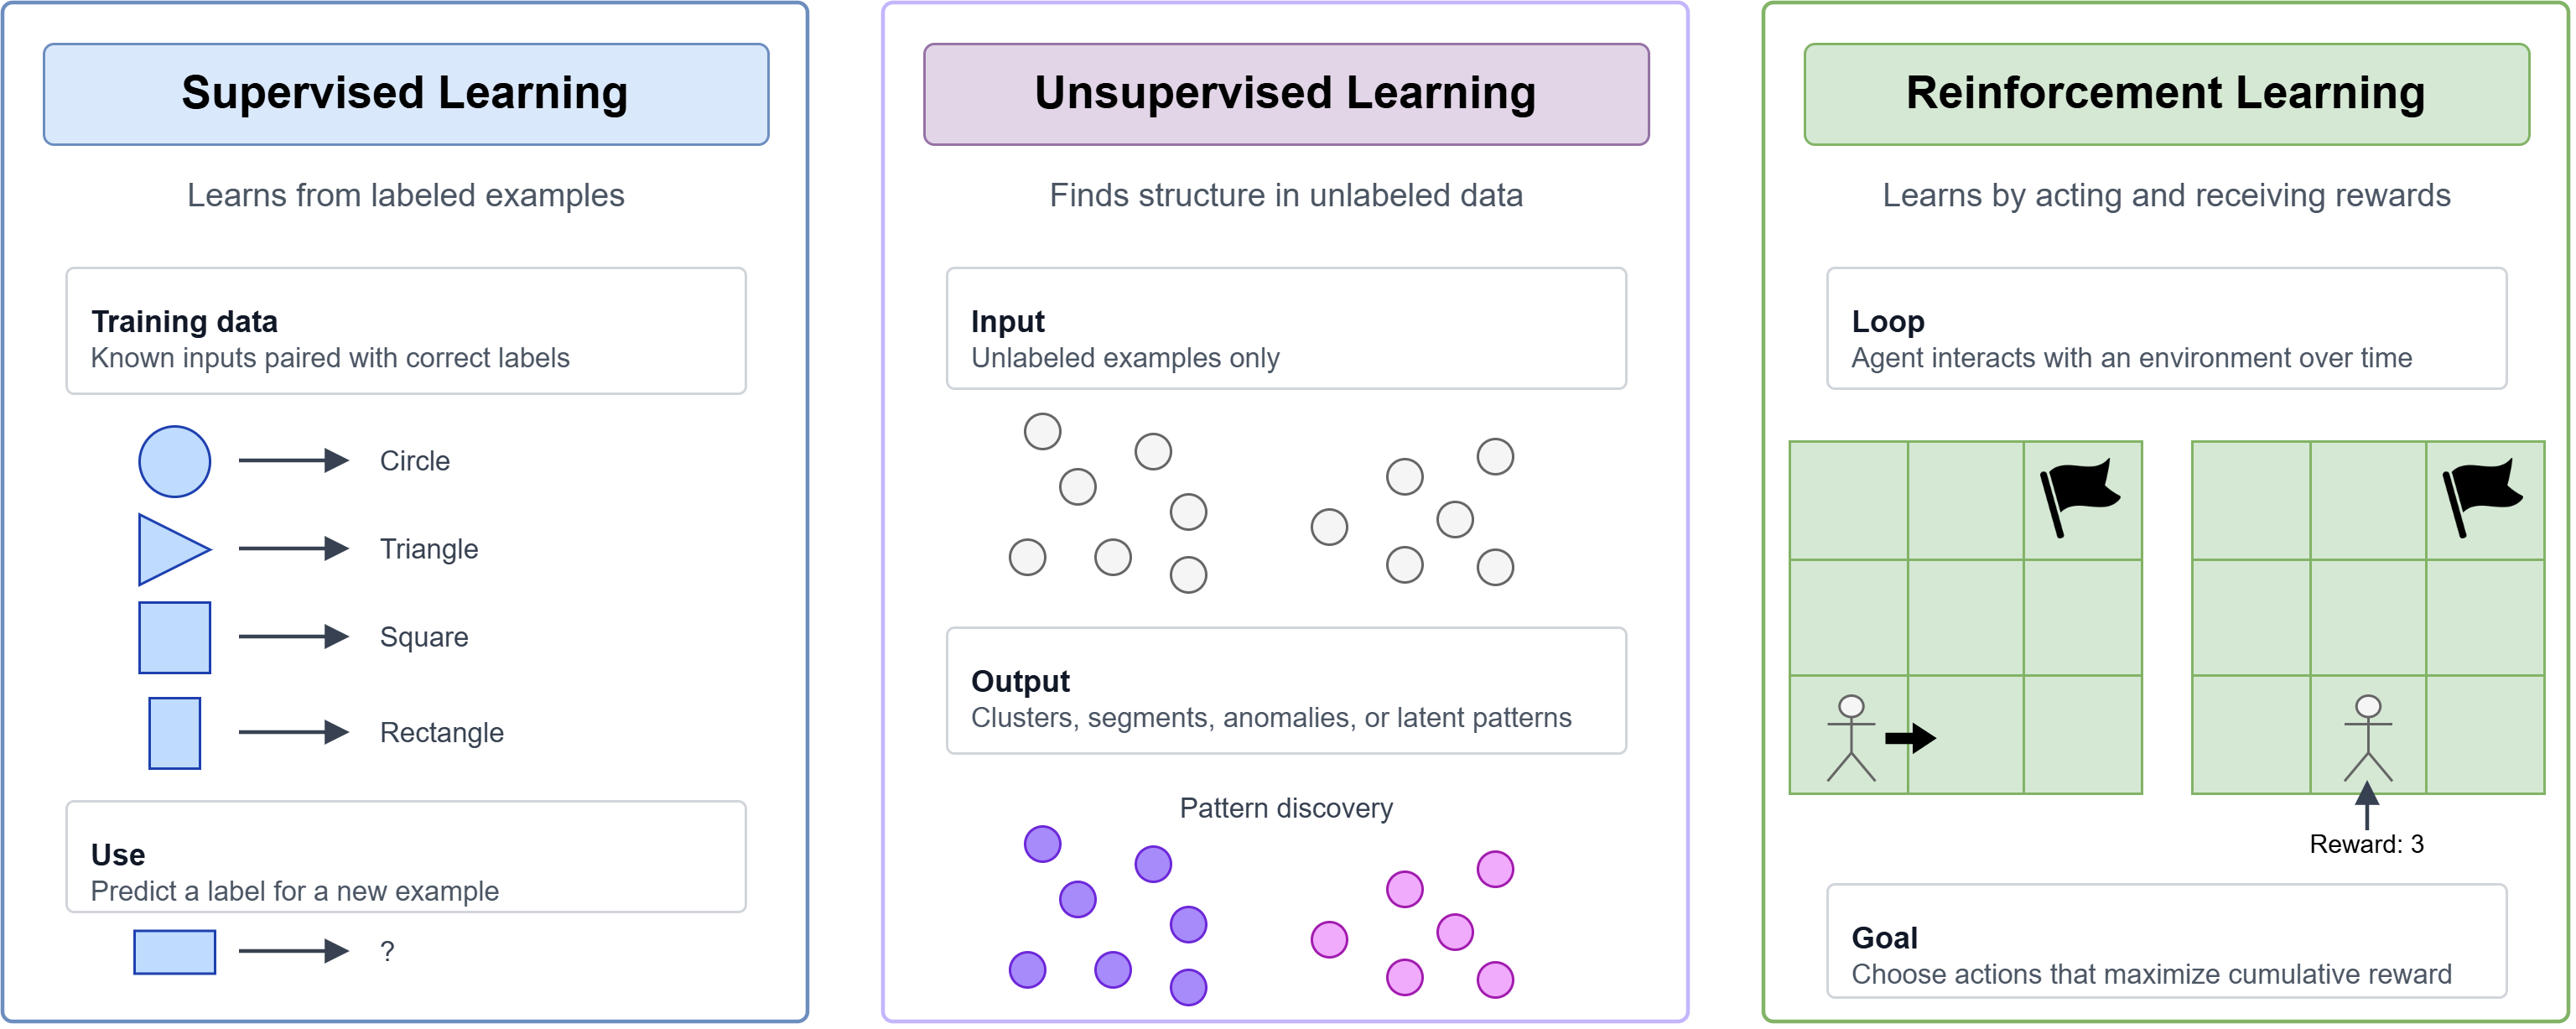
\includegraphics[width=0.96\textwidth]{images/background/learnings_example.png}
    \caption{Example of supervised, unsupervised and reinforcement learning}
    \label{fig:learnings_example}
\end{figure}

When the goal is to learn a function that maps inputs to correct outputs (labels), based on example input-output pairs, then supervised learning is useful. For the training phase in supervised learning a data set with correct labelling for each input is provided. This type of learning is supervised, as the data set is put together by some knowledgeable supervisor who will then observe how well the model predicts the labels \cite{rl_introduction}. 
Figure \ref{fig:learnings_example} demonstrates an example of supervised learning. The model receives a list of labelled data, a mapping of geometrical shapes and their names, and it uses this data to train. Once the model is trained, it labels new shapes using the knowledge it gained from the training data. Depending on the types of labels, supervised learning problems are categorised as either classification (when the label is a discrete category, as in the shape example) or regression (when the label is a continuous value) \cite{statisticalLearning}. Forecasting is a common application of regression. The model learns a mapping from time (and possibly other features) to a continuous predicted value (e.g. forecasting the weather for the next hours as seen in Section \ref{sec:application-power-grids}).

When the data is unlabelled and the goal is to find structure behind the data that might not be visible, then it is called unsupervised learning \cite{rl_introduction}. For example the unlabelled data seen in Figure \ref{fig:learnings_example}, where each data point is scattered around a two-dimensional plane. The model searches for a structure in this data, by choosing labels for each of the data points. In this case the cluster on the left and the cluster on the right are recognised and grouped, giving each point in each cluster a label (showcased as colour in the example), with each point in one cluster having the same label.

\ac{rl} takes a different approach in learning, as it is an optimisation problem seeking to improve a strategy $\pi$, called policy, to maximise reward. In Figure \ref{fig:learnings_example} the goal of the \ac{rl} agent is to move to the finish line. Every time the agent moves and lands in a new state a reward is returned. In this example the reward should be minimised, as the reward is the distance to the finish line. Hence, whenever the agent moves away from the finish line, a worse reward value will be returned, signalling to the agent, that it is moving away from the goal. As seen, \ac{rl} agents are interactive and goal-directed \cite{rl_introduction}, making decisions sequentially and learning with the reward to improve the actions selected by the agent. Supervised and unsupervised learning, however, have a fixed dataset and do not interact with any environment. The next section will explain in more detail how \ac{rl} is structured.


% ++++++++++++++++++++++++++++++++++++++++++++++++++++++++++++
\subsection{Reinforcement Learning Terminology}\label{ssec:rl-terminology}
This section summarises the key terminology of \ac{rl}, providing the formal framework and vocabulary necessary to understand the algorithms discussed later in this thesis. Based on the intuitive introduction to \ac{rl} given in Section \ref{ssec:fields-learning}, the following definitions formalise the concepts of states, actions, rewards and policies that form the basis of the interaction between an agent and its environment. The main source of the definitions of this section comes from \citet{rl_introduction}.

The environment of \ac{rl} is often modelled as a \ac{mdp}, which is a tuple that generally has the elements $\langle \mathcal{S}, \mathcal{A}, \mathcal{T}, \mathcal{R}, \gamma \rangle$. 
$\mathcal{S}$ represents the possible states of the environment, some states are also terminal (e.g. in cases of violation or exceeding a limit of the environment). A state contains the complete, exact description of the environment at a given time. In some cases, however, the agent does not have access to the full state, but only to an observation of it. This contains partial information about the state and models what the agent actually perceives of the environment \cite{openaiRLIntro}. Such settings are formally modelled as a \ac{pomdp} rather than a standard \ac{mdp} \cite{pomdp}. $\mathcal{A}$ represents the action space, while $\mathcal{T}$ describes the dynamics of the environment. Formally, $\mathcal{T}(s',r|s,a) = \Pr\{S_{t+1}=s', R_{t+1}=r \mid S_t=s, A_t=a\}$ is the joint probability of transitioning to state $s'$ and receiving reward $r$, given that the agent is in state $s$ and takes action $a$. From this, the state-transition probabilities are derived as $p(s'|s,a) = \sum_{r \in \mathcal{R}} \mathcal{T}(s',r|s,a)$, describing the probability of reaching state $s'$ given state $s$ and action $a$.
For a state $S_t \in \mathcal{S}$ in the timestep $t$, the agent selects one possible action $A_t \in \mathcal{A}$. This leads to the state $S_{t+1} \in \mathcal{S}$ and the reward $R_{t+1} \in \mathcal{R} \subset \mathbb{R}$, sampled according to $\mathcal{T}$. The reward is an immediate feedback to the agent on its decision.
Figure \ref{fig:rl-loop} shows these steps that are part of the whole \ac{rl} loop for each timestep $t$. For each step the agent receives the new state and reward and decides the next action. 
The factor $0 \le \gamma \le 1$, also called discount factor, balances the importance of future rewards against immediate ones. This is used for the discounted return 
\[G_t = R_{t+1} + \gamma R_{t+2} + \gamma^2 R_{t+3} + \cdots = \sum_{k=0}^{\infty} \gamma^k R_{t+k+1}\] 
where $\gamma^{k}$ defines how much weight a reward received $k$ timesteps in the future has. In a finite \ac{mdp} there is the horizon $H$, which defines the length of an episode, where the timesteps are defined as $0 \le t \le H$. 

\begin{figure}[htp]
    \centering
    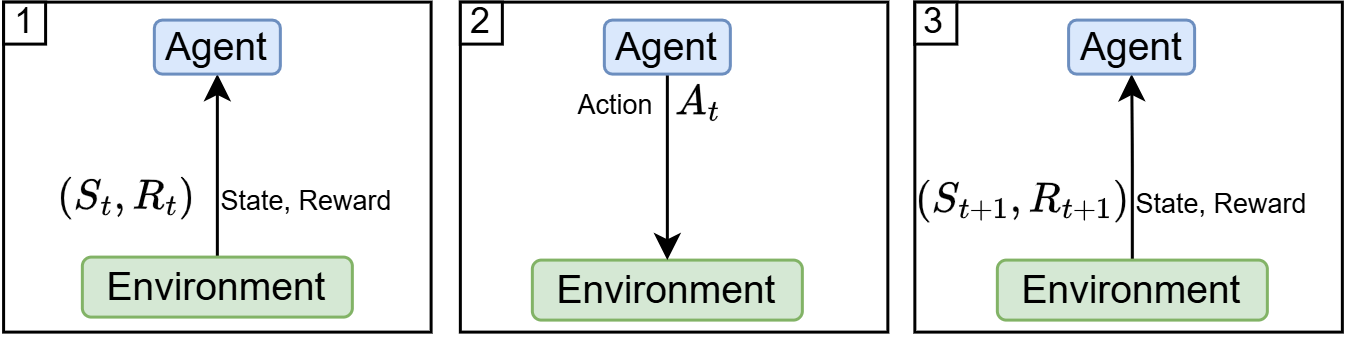
\includegraphics[width=0.8\textwidth]{images/background/RL_loop.png}
    \caption{Steps of the \ac{rl} loop at timestep $t$}
    \label{fig:rl-loop}
\end{figure}

The agent's \textbf{policy} $\pi:\mathcal{S} \times \mathcal{A} \rightarrow [0,1]$ represents the decision-making strategy that the agent follows. Simply said the policy is a mapping that decides for each state, with what probability it chooses an action. If the policy is deterministic and not stochastic, it creates a direct mapping from state to action to take \cite{openaiRLIntro}. While the reward is an immediate feedback, on the long run the \textbf{value function} $v_{\pi}(s)$ defines how favourable a state is for the agent. It defines for the agent how favourable the current state $s$ is under policy $\pi$ for future timesteps, expressed as the expected cumulative reward. The formal definition is
\[v_{\pi}(s) = \mathbb{E}_{\pi}\!\left[ G_t \mid S_t = s \right]\]
with $\mathbb{E}_{\pi}\!\left[ \cdot \right]$ being the expected value given that the agent follows policy $\pi$. 
The expected return is defined as the value of taking action $a$ in state $s$ under the policy $\pi$ and is denoted as 
\[q_{\pi}(s,a) = \mathbb{E}_{\pi}\!\left[ G_t \mid S_t = s, A_t = a \right]\]
In value-based algorithms the goal is to learn and maximise expected value and return \cite{rl2grid}. In case of finite \ac{mdp}, the agent's goal is to maximise the expected cumulative discounted sum of rewards over these timesteps \cite{grl4powergrids}.

For learning the agent's strategy, there are two approaches in \ac{rl}. For \textbf{on-policy} algorithms, they learn and update their policy through actions taken by their own policy. In each step the policy decides the next action and with the resulting data, the same policy is updated. 
\textbf{Off-policy}, on the other hand, uses two policies. The target policy is the policy that is being learned and improved, while the behaviour policy controls the agent's actions and generates the data that is used to update the target policy. As the target policy differs from the behaviour policy that generates the data, off-policy algorithms learn from data collected by any policy. This includes past versions of the behaviour policy. This is unlike on-policy algorithms, which require data generated by the exact policy being updated.

For the next immediate timesteps, \ac{rl} systems may also utilize a model of the environment, which simulates its behaviour and enables predictions of how it responds. It can be used to predict the reward, depending on a state and action that was chosen. \ac{rl} systems that use these models are called \textbf{model-based} and those without are known as \textbf{model-free}. Model-based learners plan ahead, while model-free systems are trial-and-error learners. 

Another parameter that needs to be chosen in a \ac{rl} algorithm is whether the agent favours \textbf{exploration} or \textbf{exploitation}. When the agent favours exploration, it aims to visit new states to discover more about the environment. As for exploitation, the agent uses the current knowledge to maximise reward in each step. Exploration provides insights into the environment, expanding the knowledge that the agent collects about it. Exploitation uses this knowledge to improve the agent's strategy. This illustrates the exploration-exploitation dilemma. Relying solely on exploration prevents the agent from exploiting its accumulated knowledge, while relying solely on exploitation prevents it from discovering potentially better actions. Thus it is important to find a suitable balance between these two approaches, in order that the agent continues to learn and improve itself.

% ++++++++++++++++++++++++++++++++++++++++++++++++++++++++++++
\subsection{Example Agents}\label{ssec:example-agents}
One simple example of an agent is a \textbf{greedy} agent. The following equation defines its strategy. 
\[A_t \doteq \underset{a}{\arg\max}\, q_t(s_t, a)\]
Here, $A_t$ is the action selected at timestep $t$, and $q_t(s_t, a)$ is the agent's current estimate of the value of taking action $a$ in state $s_t$. The greedy agent always aims to choose the action with the highest estimated value. 
It has no explorative strategy at all, which makes the reward estimation harder and less precise. When the rewards are noisy, more exploration is necessary to find an optimal action. An explorative alternative to the greedy agent is the \textbf{$\varepsilon$-greedy} algorithm, which adds randomness to the greedy agent's actions. With a probability of $\varepsilon$, the agent performs a random action, in order to explore the environment more. The higher this probability, the more explorative and less exploitative the agent becomes \cite{rl_introduction}, illustrating the exploration-exploitation dilemma introduced in Section \ref{ssec:rl-terminology}.

\subsubsection{Value-based agents}
A classical value-based algorithm is \textbf{Q-Learning}. It aims to improve the policy by updating values in a Q-table using an off-policy approach. This is a lookup table where each entry $q(s,a)$ is a heuristic for how favourable it is to take action $a$ in state $s$. The goal is to create a heuristic for the optimal action-value function
\[q^*(s,a) = \mathbb{E}_{\pi}\!\left[ R_{t+1} + \gamma\ \max_a\ q(S_{t+1}, a) \mid S_t = s, A_t = a \right]\]
which is the Bellman optimality equation in an action-value form \cite{foundationsRL}. This is achieved by improving the lookup table iteratively. The needed information for this is $(s_t,a_t,r_{t+1},s_{t+1})$, where $a_t$ is derived from the behaviour policy and a system model generates $r_{t+1}$ and $s_{t+1}$. The update of the Q-table is done with the following function 
\[
q_{t+1}(s_t,a_t) \leftarrow q_t(s_t,a_t) - \alpha_t(s_t,a_t)
\Big[q_t(s_t,a_t) - (r_{t+1} + \gamma \max_a q_t(s_t,a))\Big]
\]
with $q_t(s_t,a_t)$ being the current estimation on how favourable action $a_t$ is in state $s_t$ is, $\max_a q_t(s_t,a)$ as the best estimated value of the next state and $\alpha_t(s_t,a_t)$ being the learning rate, controlling the update magnitude \cite{foundationsRL}. In summary, the update can be summarised as
\[
\text{new estimate} = \text{old estimate} + \text{step size} \times \text{error}
\]
thus, the current estimate is moved towards a better estimate using the current error. The target policy is then updated with 
\[
\pi_{t+1}(a \mid s_t) =
\begin{cases}
1 & \text{if } a = \arg\max_a q_{t+1}(s_t, a), \\
0 & \text{otherwise}
\end{cases}
\quad \text{\cite{foundationsRL}.}
\]

A variation of this is \textbf{\ac{dqn}}, which uses a deep neural network to approximate the Q-values \cite{grl4powergrids}. In general, \ac{rl} algorithms that use a deep neural network to represent their policy, value function or model of the environment are called \ac{drl} algorithms. They combine deep learning with \ac{rl} \cite{deepRLIntro}.

\subsubsection{Policy-based}
A pure policy-based algorithm is \textbf{Monte Carlo Policy Gradient (REINFORCE)}. It uses a parameterised stochastic policy $\pi_\theta$ and its goal is to maximise $J(\theta)$, which is the expected return under $\pi_\theta$. For each episode of the algorithm, a trajectory $\{s_0,a_0,r_1,...,s_T\}$ is generated using the current policy $\pi_\theta$. Then the policy is improved by iterating over all $t=0,...,T-1$. This is done by first updating the value with 
\[
    q_t(s_t, a_t) = \sum_{k=t+1}^{T} \gamma^{\,k-t-1} r_k
\]
which is the return from time $t$. This is used for the Monte Carlo estimation $q_\pi(s_t,a_t) \approx q_t(s_t, a_t)$ of the action-value function under policy $\pi$ \cite{foundationsRL}. To update the policy the function
\[
\theta \leftarrow \theta + \alpha \, \nabla_\theta \ln \pi_\theta(a_t \mid s_t)\, q_t(s_t, a_t)
\]
is used \cite{foundationsRL}. $\alpha$ is the learning rate, which defines the size of the update steps, and $\nabla_\theta$ is the gradient operator. When the return from time $t$ $q_t(s_t, a_t)$ is high, the probability of $a_t$ is increased, when it is low it will be decreased. The gradient $\nabla_\theta \ln \pi_\theta(a_t \mid s_t)$ is a vector, which gives a direction. Moving to that direction increases the probability of choosing $a_t$ in state $s_t$ \cite{rl_introduction}.

\textbf{Actor-Critic} is a policy- and value-based hybrid. The algorithm contains an actor, which learns policies to maximise rewards, and a critic, which evaluates the policies from the actor, by estimating the value function. This balances pure policy methods and pure value function methods. While the critic stabilises learning, the actor handles action selection. Variations of this are the \textbf{\ac{a3c}} and \textbf{\ac{ppo}} algorithms. In \ac{a3c} multiple agents run in parallel. While each agent collects experience independently a shared global model is updated asynchronously. In the case of \ac{ppo}, the policy updates are clipped in order to stabilise the training process by preventing large jumps in the policy, which could otherwise lead to oscillations \cite{grl4powergrids}.



% ============================================================
% ============================================================
\section{Benchmarks}\label{sec:benchmarks}
This section defines benchmarks and the principles to follow when creating them. 
Benchmarks are extremely important in development and research because they provide a shared reference point that clearly defines how improvement is measured. This standardised evaluation makes results interpretable and comparable across projects and teams \cite{mlperf_benchmark,ml_benchmarks}.
This drives progress when benchmarks and their results are published. It leads to competition between multiple developers and, furthermore, helps with improvement in research \cite{mlperf_benchmark, ml_benchmarks, building_benchmarks4models}.
Benchmarks are also used to compare specific aspects. For example, a benchmark that evaluates machine learning models could be used to compare different models, training configurations, or hardware systems \cite{ml_benchmark_design}.
This comparability also supports decision-making by indicating which evaluated inputs to use in the real world \cite{building_benchmarks4models}. 
Furthermore, benchmarks make it easy for inexperienced people to understand what constitutes strong or weak performance in the evaluated field \cite{building_benchmarks4models}. 

Section \ref{sec:rw-benchmarking} provides some examples of implemented benchmarks. It shows how the benchmarks are structured for different reinforcement learning and power grid scenarios.


% ++++++++++++++++++++++++++++++++++++++++++++++++++++++++++++
\subsection{Structure of a Benchmark}\label{ssec:structure-benchmark}
Figure \ref{fig:general-benchmark} shows a general structure that every benchmark shares. In simplified terms, a benchmark is an algorithm that reads an input and returns a rating of the input using one or more scores. Benchmarks come in many forms, as they are used in a variety of different fields, in and outside of science. Even in the same field benchmarks have many forms. While a \textbf{micro-benchmark} evaluates a specific component of a benchmarked entity, a \textbf{macro-benchmark} analyses a specific task and how well this entity performs in it. An \textbf{end-to-end benchmark}, on the other hand, evaluates how an entity performs in total, from start to finish \cite{ml_benchmark_design}.

As Figure \ref{fig:general-benchmark} demonstrates, a benchmark algorithm consists of multiple components. Firstly, in order to evaluate the input, the benchmark requires data or configurations that form part of its context. The data needed in a macro- or micro-benchmark covers much less of the input's context than an end-to-end benchmark, as the latter covers a much broader scope. In the macro- and micro-benchmark the data is specialised in one aspect of the input's context. Specified tasks are then performed on these data or with these configurations, to test the behaviour of the input in different situations. For each task, metrics are measured, which are evaluated by a scoring function. This function may use a baseline or reference values to convert the measured metrics into a specific score. Finally, the output is created by using the calculated scores or by aggregating them (e.g. by computing the average value).

\begin{figure}[htp]
    \centering
    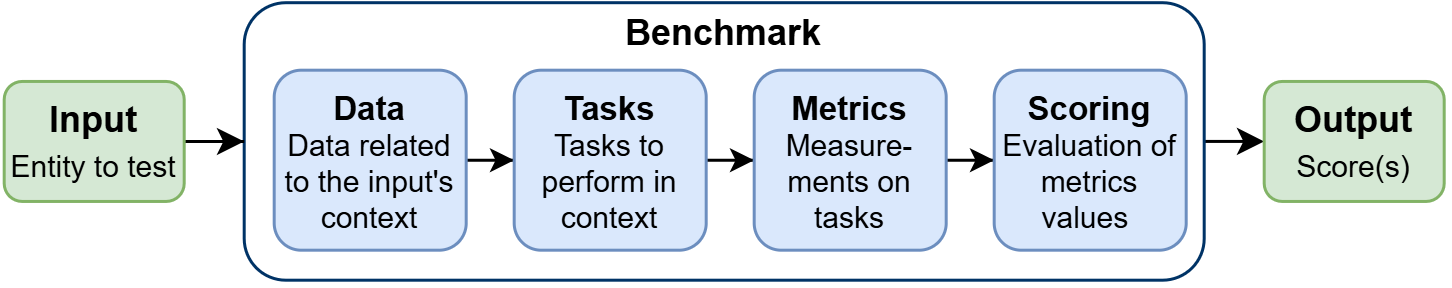
\includegraphics[width=0.8\textwidth]{images/background/general_benchmark_overview.png} 
    \caption{General structure of a benchmark}
    \label{fig:general-benchmark}
\end{figure}

% ++++++++++++++++++++++++++++++++++++++++++++++++++++++++++++
\subsection{Principles of a Benchmark}\label{ssec:principles-benchmark}
In order to construct a benchmark, there exists a series of principles that must be followed. In their absence, the relevance of a benchmark might be questionable, and its capacity to drive progress in the field might be limited. This section will provide a comprehensive overview of the fundamental principles that must be observed when constructing a benchmark, to ensure its quality. 

\paragraph{Definition of the Objective.} 
It is essential to define the objectives of the benchmark prior to its development. It must be clear what kind of goals or improvements the benchmark wants to achieve (e.g. cost-efficiency, quality of input-entity, speed or computational efficiency, etc.). By establishing these criteria at the initiation of the process, it is clear which data, tasks and metrics to use and which ones are not relevant. With this, the benchmark is precise with the resources it is using, not omitting anything important and not using any unneeded resources. 

\paragraph{Reproducibility.}
The utilisation of a benchmark must ensure reproducibility, thereby guaranteeing that the same input always yields the same output score. This is of fundamental importance for the reliability and comparability with other inputs. Certain benchmarks select context and tasks at random for a given input. This approach is appealing as it allows for the testing of diverse scenarios in each iteration, though it complicates the comparison of different inputs. In this particular instance, it is necessary for the benchmark to include a configurable seed, thus enabling the testing of two distinct inputs using the same seed and, by consequence, the same scenarios. Furthermore, reproducibility is ensured by creating a standardised evaluation algorithm. The data, tasks, metrics and scoring inside the benchmark must always follow a fixed and predefined structure.

\paragraph{Comparability.}
The ability to make meaningful comparisons is a crucial aspect of establishing a high-quality benchmark. Without the implementation of effective comparability measures, it is challenging for users to identify the most effective input or to determine whether they were enhancing the benchmarked inputs. Comparability does not necessarily imply that it is obvious which input was the best. Two different inputs may have their own strengths and weaknesses and perform better in certain scenarios than others. 

\paragraph{Transparency.}
If the benchmark is built transparently, so that the user understands how the output scoring is being calculated, it becomes more comprehensible, what the strengths and weaknesses of each input are. Perhaps one input is suitable for a specific task, or perhaps it performs perfectly in general but has some weaknesses. To achieve transparency, the outcomes of the benchmark must be interpretable, so that users can understand what the scores mean, how they are calculated, and how they relate to the performance of the input. With sufficient transparency and reproducibility, users can get a clear idea of how their inputs perform, which one to use in which situation, and which aspects to improve.

\paragraph{Relevance.}
A benchmark must be relevant to the field in which it is used. The evaluation data has to be reliable, representing the context in which the inputs are tested and aligning with real-world scenarios in which the inputs are used. Otherwise, the inputs will not encounter the problems and challenges present in real applications. 

\paragraph{Representativeness.}
Furthermore, the benchmark must be representative, meaning diverse scenarios and edge cases have to be covered to ensure the inputs are suitable for all use cases. Of course, this depends on what the benchmark tests. If it is a very specific test (e.g. a macro-benchmark, as described in \cite{ml_benchmark_design}), then the scenarios may be very similar, as the evaluation focuses on one aspect. However, if the benchmark tests generalisation and how well the inputs behave in different scenarios, it must be free from bias and ensure a fair comparison between different approaches.